%
% orthogonal.tex
%
% (c) 2021 Prof Dr Andreas Müller, OST Ostschweizer Fachhochschule
%
\section{Orthogonalität
\label{buch:integral:section:orthogonale-polynome}}
\rhead{Orthogonale Polynome}
Die Fourier-Theorie basiert auf der Idee, Funktionen durch 
Funktionenreihen mit Summanden zu bilden, die im Sinne eines
Skalarproduktes orthogonal sind, welches mit Hilfe eines Integrals
definiert sind.
Solche Funktionenfamilien treten jedoch auch als Lösungen von
Differentialgleichungen.
Besonders interessant wird die Situation, wenn die Funktionen 
Polynome sind.

%
% Skalarprodukt
%
\subsection{Skalarprodukt}
Der reelle Vektorraum $\mathbb{R}^n$ trägt das Skalarprodukt
\[
\langle\;\,,\;\rangle
\colon
\mathbb{R}^n \times \mathbb{R}^n \to \mathbb{R}
:
(x,y)\mapsto \langle x, y\rangle = \sum_{k=1}^n x_iy_k,
\]
welches viele interessante Anwendungen ermöglicht.
Eine orthonormierte Basis macht es zum Beispiel besonders leicht,
eine Zerlegung eines Vektors in dieser Basis zu finden.
In diesem Abschnitt soll zunächst an die Eigenschaften erinnert
werden, die zu einem nützlichen 

\subsubsection{Eigenschaften eines Skalarproduktes}
Das Skalarprodukt erlaubt auch, die Länge eines Vektors $v$
als $|v| = \sqrt{\langle v,v\rangle}$ zu definieren.
Dies funktioniert natürlich nur, wenn die Wurzel auch immer
definiert ist, d.~h.~das Skalarprodukt eines Vektors mit sich
selbst darf nicht negativ sein.
Dazu dient die folgende Definition.

\begin{definition}
Sei $V$ ein reeller Vektorraum.
Eine bilineare Abbildung
\[
\langle\;\,,\;\rangle
\colon
V\times V
\to
\mathbb{R}
:
(u,v) \mapsto \langle u,v\rangle.
\]
heisst {\em positiv definit}, wenn für alle Vektoren $v \in V$ mit
$v\ne 0 \Rightarrow \langle v,v\rangle > 0$ 
Die {\em Norm} eines Vektors $v$ ist
$|v|=\sqrt{\langle v,v\rangle}$.
\end{definition}

Damit man mit dem Skalarprodukt sinnvoll rechnen kann, ist ausserdem
erforderlich, dass es eine einfache Beziehung zwischen 
$\langle x,y\rangle$ und $\langle y,x\rangle$ gibt.

\begin{definition}
Ein {\em Skalarprodukt} auf einem reellen Vektorraum $V$ ist eine
positiv definite, symmetrische bilineare Abbildung
\[
\langle\;\,,\;\rangle
\colon
V\times V
\to
\mathbb{R}
:
(u,v) \mapsto \langle u,v\rangle.
\]
\end{definition}

Das Skalarprodukt $\langle u,v\rangle=u^tv$ auf dem Vektorraum 
$\mathbb{R}^n$ erfüllt die Definition ganz offensichtlich,
sie führt auf die Komponentendarstellung
\[
\langle u,v\rangle = u^tv = \sum_{k=1}^n u_iv_i.
\]
Weitere Skalarprodukte ergeben ergeben sich mit jeder symmetrischen,
positiv definiten Matrix $G$ und der Definition
$\langle u,v\rangle_G=u^tGv$.
Ein einfacher Spezialfall tritt auf, wenn $G$ eine Diagonalmatrix
$\operatorname{diag}(w_1,\dots,w_n)$
mit positiven Einträgen $w_i>0$ auf der Diagonalen ist.
In diesem Fall schreiben wir
\[
\langle u,v\rangle_w
=
u^t\operatorname{diag}(w_1,\dots,w_n)v
=
\sum_{k=1}^n u_iv_i\,w_i
\]
und nennen $\langle \;\,,\;\rangle_w$ das {\em gewichtete Skalarprodukt}
mit {\em Gewichten $w_i$}.

\subsubsection{Skalarprodukte auf Funktionenräumen}
Das Integral ermöglicht jetzt, ein Skalarprodukt auf dem reellen
Vektorraum der stetigen Funktionen auf einem Intervall zu definieren.

\begin{definition}
Sei $V$ der reelle Vektorraum $C([a,b])$ der reellwertigen, stetigen
Funktion auf dem Intervall $[a,b]$.
Dann ist 
\[
\langle\;\,,\;\rangle
\colon
C([a,b]) \times C([a,b]) \to \mathbb{R}
:
(f,g) \mapsto \langle f,g\rangle = \int_a^b f(x)g(x)\,dx.
\]
ein Skalarprodukt.
\end{definition}

Die Definition ist offensichtlich symmetrisch in $f$ und $g$ und
aus den Eigenschaften des Integrals ist klar, dass das Produkt
bilinear ist:
\begin{align*}
\langle \lambda_1 f_1+\lambda_2f_2,g\rangle
&=
\int_a^b (\lambda_1f_(x) +\lambda_2f_2(x))g(x)\,dx
=
\lambda_1\int_a^b f_1(x) g(x)\,dx
+
\lambda_2\int_a^b f_2(x) g(x)\,dx
\\
&=
\lambda_1\langle f_1,g\rangle
+
\lambda_2\langle f_2,g\rangle.
\end{align*}
Ausserdem ist es positiv definit, denn wenn $f(x_0) \ne 0$ ist,
dann gibt es wegen der Stetigkeit von $f$ eine Umgebung
$U=[x_0-\varepsilon,x_0+\varepsilon]$, derart, dass $|f(x)| > \frac12|f(x_0)|$
ist für alle $x\in U$.
Somit ist das Integral
\[
\langle f,f\rangle
=
\int_a^b |f(x)|^2\,dx
\ge
\int_{x_0-\varepsilon}^{x_0+\varepsilon} |f(x)|^2\,dx
\ge
\int_{x_0-\varepsilon}^{x_0+\varepsilon} \frac14|f(x_0)|^2\,dx
=
\frac{1}{4}|f(x_0)|^2\cdot 2\varepsilon
=
\frac{|f(x_0)|\varepsilon}{2}
>0,
\]
was beweist, dass $\langle\;,\;\rangle$ positiv definit und damit
ein Skalarprodukt ist.

Die Definition kann noch etwas verallgemeinert werden, indem 
die Funktionswerte nicht überall auf dem Definitionsbereich 
gleich gewichtet werden. 

\begin{definition}
Sei $w\colon [a,b]\to \mathbb{R}^+$ eine positive, stetige Funktion,
dann ist
\[
\langle\;\,,\;\rangle_w
\colon
C([a,b]) \times C([a,b]) \to \mathbb{R}
:
(f,g) \mapsto \langle f,g\rangle_w = \int_a^b f(x)g(x)\,w(x)\,dx.
\]
das {\em gewichtete Skalarprodukt} mit {\em Gewichtsfunktion $w(x)$}.
\end{definition}

\subsubsection{Gram-Schmidt-Orthonormalisierung}
In einem reellen Vektorraum $V$ mit Skalarprodukt $\langle\;\,,\;\rangle$
kann aus einer beleibigen Basis $b_1,\dots,b_n$ mit Hilfe des 
Gram-Schmidtschen Orthogonalisierungsverfahrens immer eine
orthonormierte Basis $\tilde{b}_1,\dots,\tilde{b}_n$ Basis
gewonnen werden.
Es stellt sicher, dass für alle $k\le n$ gilt
\[
\langle b_1,\dots,b_k\rangle
=
\langle \tilde{b}_1,\dots,\tilde{b}_k\rangle.
\]
Zur Vereinfachung der Formeln schreiben wir $v^0=v/|v|$ für einen zu
$v$ parallelen Einheitsvektor.
Die Vektoren $\tilde{b}_i$ können mit Hilfe der Formeln
\begin{align*}
\tilde{b}_1
&=
(b_1)^0
\\
\tilde{b}_2
&=
\bigl(
b_2
-
\langle \tilde{b}_1,b_2\rangle \tilde{b}_1
\bigr)^0
\\
\tilde{b}_3
&=
\bigl(
b_3
-
\langle \tilde{b}_1,b_3\rangle \tilde{b}_1
-
\langle \tilde{b}_2,b_3\rangle \tilde{b}_2
\bigr)^0
\\
&\;\vdots
\\
\tilde{b}_n
&=
\bigl(
b_n
-
\langle \tilde{b}_1,b_n\rangle \tilde{b}_1
-
\langle \tilde{b}_2,b_n\rangle \tilde{b}_2
-\dots
-
\langle \tilde{b}_{n-1},b_n\rangle \tilde{b}_{n-1}
\bigr)^0
\end{align*}
iterativ berechnet werden.
Dieses Verfahren lässt sich auch auf Funktionenräume anwenden.

Die Normierung ist nicht unbedingt nötig und manchmal unangenehm,
da die Norm unschöne Quadratwurzeln einführt.
Falls es genügt, eine orthogonale Basis zu finden, kann darauf
verzichtet werden, bei der Orthogonalisierung muss aber berücksichtigt
werden, dass die Vektoren $\tilde{b}_i$ jetzt nicht mehr Einheitslänge
haben.
Die Formeln
\begin{align*}
\tilde{b}_0
&=
b_0
\\
\tilde{b}_1
&=
b_1
-
\frac{\langle b_1,\tilde{b}_0\rangle}{\langle \tilde{b}_0,\tilde{b}_0\rangle}\tilde{b}_0
\\
\tilde{b}_2
&=
b_2
-
\frac{\langle b_2,\tilde{b}_0\rangle}{\langle \tilde{b}_0,\tilde{b}_0\rangle}\tilde{b}_0
-
\frac{\langle b_2,\tilde{b}_1\rangle}{\langle \tilde{b}_1,\tilde{b}_1\rangle}\tilde{b}_1
\\
&\;\vdots
\\
\tilde{b}_n
&=
b_n
-
\frac{\langle b_n,\tilde{b}_0\rangle}{\langle \tilde{b}_0,\tilde{b}_0\rangle}\tilde{b}_0
-
\frac{\langle b_n,\tilde{b}_1\rangle}{\langle \tilde{b}_1,\tilde{b}_1\rangle}\tilde{b}_1
-
\dots
-
\frac{\langle b_n,\tilde{b}_{n-1}\rangle}{\langle \tilde{b}_{n-1},\tilde{b}_{n-1}\rangle}\tilde{b}_{n-1}.
\end{align*}
berücksichtigen dies.

\subsubsection{Selbstadjungierte Operatoren und Eigenvektoren}
Symmetrische Matrizen spielen eine spezielle Rolle in der
endlichdimensionalen linearen Algebra, weil sie sich immer
mit einer orthonormierten Basis diagonalisieren lassen.
In der vorliegenden Situation undendlichdimensionaler Vektorräume
brauchen wir eine angepasste Definition.

\begin{definition}
Eine lineare Selbstabbildung $A\colon V\to V$
eines Vektorrraums mit Skalarprodukt
heisst {\em selbstadjungiert}, wenn für alle Vektoren $u,v\in V$
heisst $\langle Au,v\rangle = \langle u,Av\rangle$.
\end{definition}

Es ist wohlbekannt, dass Eigenvektoren einer symmetrischen Matrix
zu verschiedenen Eigenwerten orthogonal sind.
Der Beweis ist direkt übertragbar, wir halten das Resultat hier
für spätere Verwendung fest.

\begin{satz}
Sind $f$ und $g$ Eigenvektoren eines selbstadjungierten Operators $A$
zu verschiedenen Eigenwerten $\lambda$ und $\mu$, dann sind $f$ und $g$
orthogonal.
\end{satz}

\begin{proof}[Beweis]
Im vorliegenden Zusammenhang möchten wir die Eigenschaft nutzen,
dass Eigenfunktionen eines selbstadjungierten Operatores zu verschiedenen
Eigenwerten orthogonal sind.
Dazu seien $Df = \lambda f$ und $Dg=\mu g$ und wir rechnen
\begin{equation*}
\renewcommand{\arraycolsep}{2pt}
\begin{array}{rcccrl}
\langle Df,g\rangle &=& \langle \lambda f,g\rangle &=& \lambda\phantom{)}\langle f,g\rangle
&\multirow{2}{*}{\hspace{3pt}$\biggl\}\mathstrut-\mathstrut$}\\
=\langle f,Dg\rangle &=& \langle f,\mu g\rangle &=& \mu\phantom{)}\langle f,g\rangle&
\\[2pt]
\hline
         0           & &                        &=& (\lambda-\mu)\langle f,g\rangle&
\end{array}
\end{equation*}
Da $\lambda-\mu\ne 0$ ist, muss $\langle f,g\rangle=0$ sein.
\end{proof}

\begin{beispiel}
Sei $C^1([0,2\pi], \mathbb{C})=C^1(S^1,\mathbb{C})$
der Vektorraum der $2\pi$-periodischen differenzierbaren Funktionen mit
dem Skalarprodukt 
\[
\langle f,g\rangle
=
\frac{1}{2\pi}\int_0^{2\pi} \overline{f(t)}g(t)\,dt
\]
enthält die Funktionen $e_n(t) = e^{int}$.
Der Operator
\[
D=i\frac{d}{dt}
\]
ist selbstadjungiert, denn mit Hilfe von partieller Integration erhält man
\[
\langle Df,g\rangle
=
\frac{1}{2\pi}
\int_0^{2\pi}
\underbrace{
\overline{i\frac{df(t)}{dt}}
}_{\uparrow}
\underbrace{g(t)}_{\downarrow}
\,dt
=
\underbrace{
\frac{-i}{2\pi}
\biggl[
\overline{f(t)}g(t)
\biggr]_0^{2\pi}
}_{\displaystyle=0}
+
\frac{1}{2\pi}
\int_0^{2\pi}
\overline{f(t)}i\frac{dg(t)}{dt}
\,dt
=
\langle f,Dg\rangle
\]
unter Ausnützung der $2\pi$-Periodizität der Funktionen.

Die Funktionen $e_n(t)$ sind Eigenfunktionen des Operators $D$, denn
\[
De_n(t) = i\frac{d}{dt}e^{int} = -n e^{int} = -n e_n(t).
\]
Nach obigem Satz sind die Eigenfunktionen von $D$ orthogonal.
\end{beispiel}

Das Beispiel illustriert, dass orthogonale Funktionenfamilien
ein automatisches Nebenprodukt selbstadjungierter Operatoren sind.

%
% Besselfunktionen also orthogonale Funktionenfamilie
%
\subsection{Bessel-Funktionen als orthogonale Funktionenfamilie}
Auch die Besselfunktionen sind eine orthogonale Funktionenfamilie.
Sie sind Funktionen differenzierbaren Funktionen $f(r)$ für $r>0$
mit $f'(r)=0$ und für $r\to\infty$ nimmt $f(r)$ so schnell ab, dass
auch $rf(r)$ noch gegen $0$ strebt.
Das Skalarprodukt ist
\[
\langle f,g\rangle
=
\int_0^\infty r f(r) g(r)\,dr,
\]
als Operator verwenden wir
\[
A = \frac{d^2}{dr^2} + \frac{1}{r}\frac{d}{dr} + s(r),
\]
wobei $s(r)$ eine beliebige integrierbare Funktion sein kann.
Zunächst überprüfen wir, ob dieser Operator wirklich selbstadjungiert ist.
Dazu rechnen wir
\begin{align}
\langle Af,g\rangle
&=
\int_0^\infty
r\,\biggl(f''(r)+\frac1rf'(r)+s(r)f(r)\biggr) g(r)
\,dr
\notag
\\
&=
\int_0^\infty rf''(r)g(r)\,dr
+
\int_0^\infty f'(r)g(r)\,dr
+
\int_0^\infty s(r)f(r)g(r)\,dr.
\notag
\intertext{Der letzte Term ist symmetrisch in $f$ und $g$, daher
ändern wir daran weiter nichts.
Auf das erste Integral kann man partielle Integration anwenden und erhält}
&=
\biggl[rf'(r)g(r)\biggr]_0^\infty
-
\int_0^\infty f'(r)g(r) + rf'(r)g'(r)\,dr
+
\int_0^\infty f'(r)g(r)\,dr
+
\int_0^\infty s(r)f(r)g(r)\,dr.
\notag
\intertext{Der erste Term verschwindet wegen der Bedingungen an die
Funktionen $f$ und $g$.
Der erste Term im zweiten Integral hebt sich gegen das
zweite Integral weg.
Der letzte Term ist das Skalarprodukt von $f'$ und $g'$.
Somit ergibt sich
}
&=
-\langle f',g'\rangle
+
\int_0^\infty s(r) f(r)g(r)\,dr.
\label{buch:integrale:orthogonal:besselsa}
\end{align}
Vertauscht man die Rollen von $f$ und $g$, erhält man das Gleiche, da im
letzten Ausdruck~\eqref{buch:integrale:orthogonal:besselsa} die Funktionen
$f$ und $g$ symmetrische auftreten.
Damit ist gezeigt, dass der Operator $A$ selbstadjungiert ist.
Es folgt nun, dass Eigenvektoren des Operators $A$ automatisch
orthogonal sind.

Eigenfunktionen von $A$ sind aber Lösungen der Differentialgleichung
\[
\begin{aligned}
&&
Af&=\lambda f
\\
&\Rightarrow\qquad&
f''(r) +\frac1rf'(r) + s(r)f(r) &= \lambda f(r)
\\
&\Rightarrow\qquad&
r^2f''(r) +rf'(r)+ (-\lambda r^2+s(r)r^2)f(r) &= 0
\end{aligned}
\]
sind.

Durch die Wahl $s(r)=1$ wird der Operator $A$ zum Bessel-Operator.
Die Lösungen der Besselschen Differentialgleichung zu verschiedenen Werten
des Parameters müssen also orthogonal sein, insbesondere sind die
Besselfunktion $J_\nu(r)$ und $J_\mu(r)$ orthogonal wenn $\mu\ne\nu$ ist.

%
% Orthogonale Polynome
%
\subsection{Orthogonale Polynome
\label{buch:integral:subsection:orthogonale-polynome}}
Die Polynome $1,x,x^2,\dots,x^n$ bilden eine Basis des Vektorraums
der Polynome vom Grad $\le n$.
Bezüglich des Skalarproduktes
\[
\langle p,q\rangle
=
\int_{-1}^1 p(x)q(x)\,dx
\]
sind sie jedoch nicht orthogonal, denn es ist
\[
\langle x^i,x^j\rangle
=
\int_{-1}^1 x^{i+j}\,dx
=
\biggl[\frac{x^{i+j+1}}{i+j+1}\biggr]_{-1}^1
=
\begin{cases}
\displaystyle
\frac{2}{i+j+1}&\qquad\text{$i+j$ gerade}\\
              0&\qquad\text{$i+j$ ungerade}.
\end{cases}
\]
Wir können daher das Gram-Schmidtsche Orthonormalisierungsverfahren
anwenden, um eine orthogonale Basis von Polynomen zu finden, was
wir im Folgenden tun wollen.

% XXX Orthogonalisierungsproblem so formulieren, dass klar wird,
% XXX dass man ein "Normierungskriterium braucht.

Da wir auf die Normierung verzichten, brauchen wir ein anderes
Kriterium, welches die Polynome eindeutig festlegen kann.
Wir bezeichnen das Polynom vom Grad $n$, das bei diesem Prozess
entsteht, mit $P_n(x)$ und legen willkürlich aber traditionskonform
fest, dass $P_n(1)=1$ sein soll.

Das Skalarprodukt berechnet ein Integral eines Produktes von zwei
Polynomen über das symmetrische Interval $[-1,1]$.
Ist die eine gerade und die andere ungerade, dann ist das
Produkt eine ungerade Funktion und das Skalarprodukt verschwindet.
Sind beide Funktionen gerade oder ungerade, dann ist das Produkt
gerade und das Skalarprodukt ist im Allgmeinen von $0$ verschieden.
Dies zeigt, dass es tatsächlich etwas zu Orthogonalisieren gibt.

Die ersten beiden Funktionen sind das konstante Polynom $1$ und
das Polynome $x$.
Nach obiger Beobachtung ist das Skalarprodukt $\langle 1,x\rangle=0$,
also ist $P_1(x)=x$.
Die Graphen der entstehenden Polynome sind in
Abbildung~\ref{buch:integral:orthogonal:legendregraphen}
dargestellt.
\begin{figure}
\centering
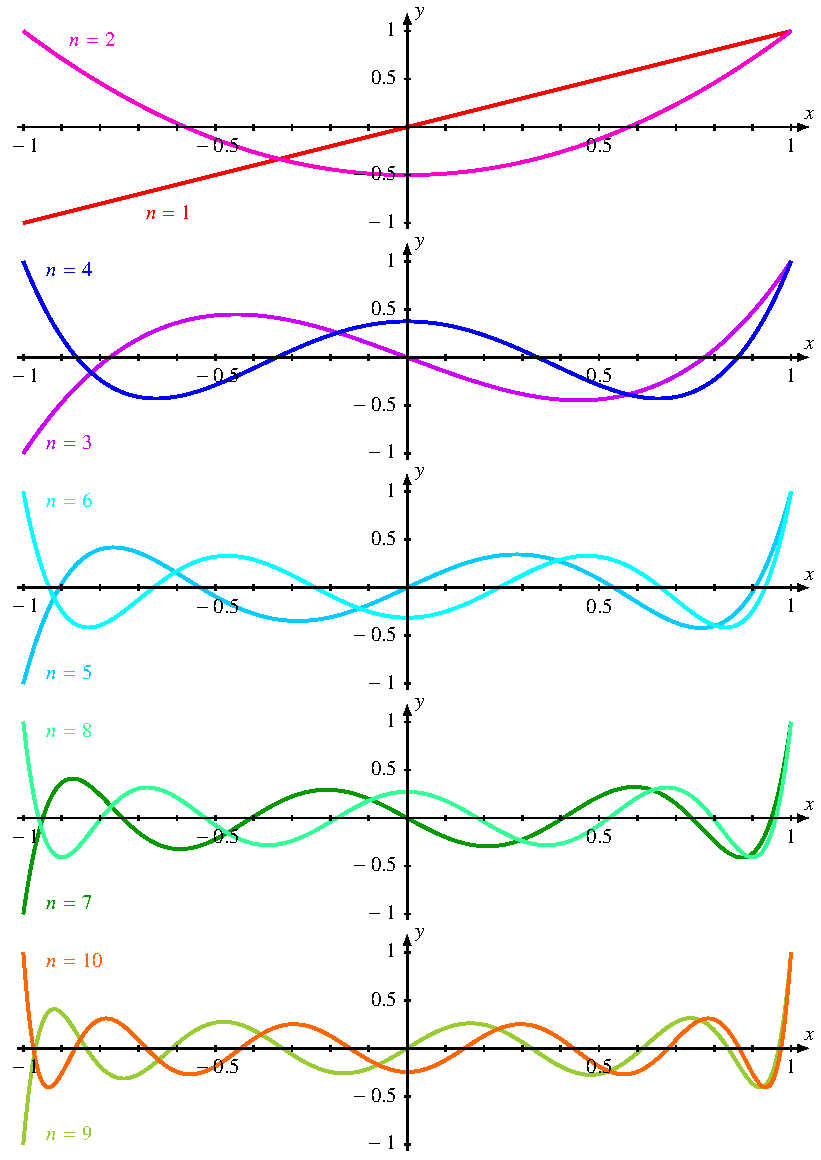
\includegraphics{chapters/060-integral/images/legendre.pdf}
\caption{Graphen der Legendre-Polynome $P_n(x)$ für $n=1,\dots,10$.
\label{buch:integral:orthogonal:legendregraphen}}
\end{figure}

\begin{lemma}
Die Polynome $P_{2n}(x)$ sind gerade, die Polynome $P_{2n+1}(x)$ sind
ungerade Funktionen von $x$.
\end{lemma}

\begin{proof}[Beweis]
Wir verwenden vollständige Induktion nach $n$.
Wir wissen bereits, dass $P_0(x)=1$ und $P_1(x)=x$ die verlangten
Symmetrieeigenschaften haben.
Im Sinne der Induktionsannahme nehmen wir daher an, dass die
Symmetrieeigenschaften für $P_k(x)$, $k<n$, bereits bewiesen sind.
$P_n(x)$ entsteht jetzt durch Orthogonalisierung nach der Formel
\[
P_n(x)
=
x^n
-
\langle P_{n-1},x^n\rangle P_{n-1}(x)
-
\langle P_{n-2},x^n\rangle P_{n-2}(x)
-\dots-
\langle P_1,x^n\rangle P_1(x)
-
\langle P_0,x^n\rangle P_0(x).
\]
Die Skalarprodukte
$\langle P_{n-1},x^n\rangle$,
$\langle P_{n-3},x^n\rangle$, $\dots$ verschwinden alle, so dass
$P_n(x)$ eine Linearkombination der Funktionen $x^n$, $P_{n-2}(x)$,
$P_{n-4}(x)$ ist, die die gleiche Parität wie $x^n$ haben.
Also hat auch $P_n(x)$ die gleiche Parität, was das Lemma beweist.
\end{proof}

Die Ortogonalisierung von $x^2$ liefert daher
\[
p(x) = x^2
-
\frac{\langle x^2,P_0\rangle}{\langle P_0,P_0\rangle} P_0(x)
=
x^2 - \frac{\int_{-1}^1x^2\,dx}{\int_{-1}^11\,dx}
=
x^2 - \frac{\frac{2}{3}}{2}=x^2-\frac13
\]
Dieses Polynom erfüllt die Standardisierungsbedingung noch 
nicht den $p(1)=\frac23$.
Daraus leiten wir ab, dass
\[
P_2(x) = \frac12(3x^2-1)
\]
ist.

Für $P_3(x)$ brauchen wir nur die Skalaprodukte
\[
\left.
\begin{aligned}
\langle x^3,P_1\rangle
&=
\int_{-1}^1  x^3\cdot x\,dx
=
\biggl[\frac15x^5\biggr]_{-1}^1
=
\frac25
\qquad
\\
\langle P_1,P_1\rangle
&=
\int_{-1}^1 x^2\,dx
=
\frac23
\end{aligned}
\right\}
\qquad
\Rightarrow
\qquad
p(x) = x^3 - \frac{\frac25}{\frac23}x=x^3-\frac{3}{5}x
\]
Die richtige Standardisierung ergibt sich,
indem man durch $p(1)=\frac25$ dividiert, also
\[
P_2(x) = \frac12(5x^3-3x).
\]

Die Berechnung weiterer Polynome verlangt, dass Skalarprodukte
$\langle x^n,P_k\rangle$ berechnet werden müssen, was wegen
der zunehmend komplizierten Form von $P_k$ etwas mühsam ist.
Wir berechnen den Fall $P_4$.
Dazu muss das Polynom $x^4$ um eine Linearkombination von
$P_2$ und $P_0(x)=1$ korrigiert werden.
Die Skalarprodukte sind
\begin{align*}
\langle x^4, P_0\rangle
&=
\int_{-1}^1 x^4\,dx = \frac25
\\
\langle P_0,P_0\rangle
&=
\int_{-1}^1 \,dx = 2
\\
\langle x^4,P_2\rangle
&=
\int_{-1}^1 \frac32x^6-\frac12 x^4\,dx
=
\biggl[\frac{3}{14}x^7-\frac{1}{10}x^5\biggr]_{-1}^1
=
\frac6{14}-\frac15
=
\frac8{35}
\\
\langle P_2,P_2\rangle
&=
\int_{-1}^1 \frac14(3x^2-1)^2\,dx
=
\int_{-1}^1 \frac14(9x^4-6x^2+1)\,dx
=
\frac14(\frac{18}{5}-4+2)
=\frac25.
\end{align*}
Daraus folgt für $p(x)$
\begin{align*}
p(x)
&=
x^4
-
\frac{\langle x^4,P_2\rangle}{\langle P_2,P_2\rangle}P_2(x)
-
\frac{\langle x^4,P_0\rangle}{\langle P_0,P_0\rangle}P_0(x)
\\
&=
x^4
-\frac47 P_2(x) - \frac15 P_0(x)
\\
&=
x^4 - \frac{6}{7}x^2 + \frac{3}{35}
\end{align*}
mit $p(1)=\frac{8}{35}$, so dass man
\[
P_4(x) =
\frac18(35x^4-30x^2+3)
\]
setzen muss.

\begin{figure}
\centering
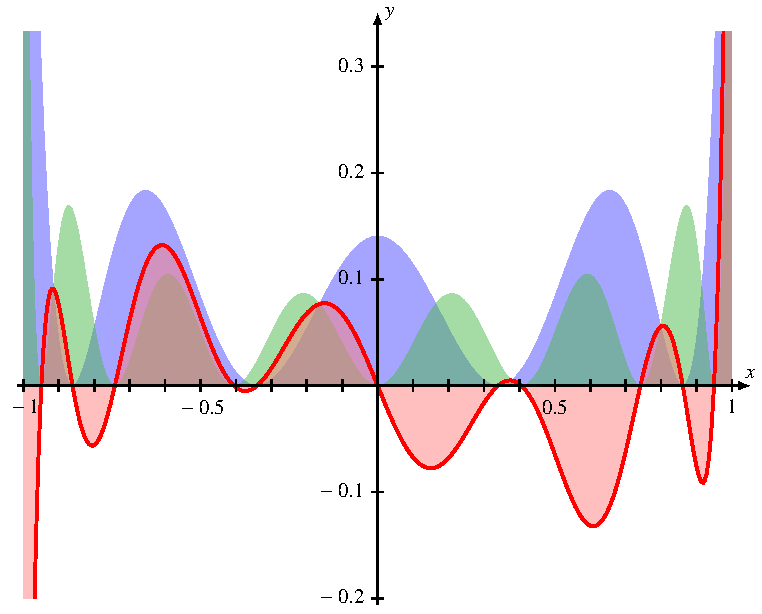
\includegraphics{chapters/060-integral/images/orthogonal.pdf}
\caption{Orthogonalität der Legendre-Polynome $P_4(x)$ ({\color{blue}blau})
und $P_7(x)$ ({\color{darkgreen}grün}).
Die blaue Fläche ist die Fläche unter dem Graphen 
von $P_4(x)^2$, $P_4(x)$ muss durch die Wurzel aus diesem Flächeninhalt
geteilt werden, um ein Polynome mit Norm $1$ zu erhalten.
Für die grüne Fläche ist es $P_7(x)$.
Die rote Kurve ist der Graph der Funktion $P_4(x)\cdot P_7(x)$,
die rote Fläche ist deren Integral, sie ist $0$, d.~h.~die beiden
Funktionen sind orthogonal.
\label{buch:integral:orthogonal:legendreortho}}
\end{figure}

\begin{table}
\centering
\renewcommand{\arraystretch}{1.2}
\begin{tabular}{|>{$}c<{$}|>{$}l<{$}|}
\hline
n&P_n(x)\\
\hline
 0&1
\\
 1&x
\\
 2&\frac12(3x^2-1)
\\
 3&\frac12(5x^3-3x)
\\
 4&\frac18(35x^4-30x^2+3)
\\
 5&\frac18(63x^5-70x^3+15x)
\\
 6&\frac1{16}(231x^6-315x^4+105x^2-5)
\\
 7&\frac1{16}(429x^7-693x^5+315x^3-35x)
\\
 8&\frac1{128}(6435x^8-12012x^6+6930x^4-1260x^2+35)
\\
 9&\frac1{128}(12155x^9-25740x^7+18018x^5-4620x^3+315x)
\\
10&\frac1{256}(46189x^{10}-109395x^8+90090x^6-30030x^4+3465x^2-63)
\\[2pt]
\hline
\end{tabular}
\caption{Die Legendre-Polynome $P_n(x)$ für $n=0,1,\dots,10$ sind
orthogonale Polynome vom Grad $n$, die den Wert $P_n(1)=1$ haben.
\label{buch:integral:table:legendre-polynome}}
\end{table}



Die so konstruierten Polynome heissen die {\em Legendre-Polynome}.
Durch weitere Durchführung des Verfahrens liefert die Polynome in
Tabelle~\ref{buch:integral:table:legendre-polynome}.
Die Graphen sind in Abbildung~\ref{buch:integral:orthogonal:legendregraphen}
dargestellt.
Abbildung~\ref{buch:integral:orthogonal:legendreortho} illustriert, 
dass die die beiden Polynome $P_4(x)$ und $P_7(x)$ orthogonal sind.
Das Produkt $P_4(x)\cdot P_7(x)$ hat Integral $=0$.


%%
%% Differentialgleichungen
%%
%\subsection{Orthogonale Polynome und Differentialgleichungen}
%\subsubsection{Legendre-Differentialgleichung}
%\subsubsection{Legendre-Polyome}
%\subsubsection{Legendre-Funktionen zweiter Art}
%Siehe Wikipedia-Artikel \url{https://de.wikipedia.org/wiki/Legendre-Polynom}

%
% legendredgl.tex
%
% (c) 2021 Prof Dr Andreas Müller, OST Ostschweizer Fachhochschule
%
\subsection{Orthogonale Polynome und Differentialgleichungen}
Legendre hat einen ganz anderen Zugang zu den nach ihm benannten
Polynomen gefunden.
Er hat sie gefunden als die Lösungen einer speziellen Differentialgleichungen.
In diesem Abschnitt sollen diese Funktionen mit der Potenzreihen-Methode
wiedergefunden werden.
Dabei stellt sich heraus, dass diese Polynome auch Eigenfunktionen eines
selbstadjungierten Differentialgoperator sind.
Die Orthogonalität wird dann aus einer Verallgemeinerung der bekannten
Eingeschaft folgen, dass Eigenvektoren einer symmetrischen Matrix zu 
verschiedenen Eigenwerten orthogonal sind.

\subsubsection{Legendre-Differentialgleichung}
Die {\em Legendre-Differentialgleichung} ist die Differentialgleichung
\begin{equation}
(1-x^2) y'' - 2x y' + n(n+1) y = 0
\label{buch:integral:eqn:legendre-differentialgleichung}
\end{equation}
für eine Funktion $y(x)$ auf dem Intervall $[-1,1]$.

Sei $y(x)$ eine Lösung der Differentialgleichung
\eqref{buch:integral:eqn:legendre-differentialgleichung}.
Setzt man $y_s(x)=y(-x)$ in die Differentialgleichung ein, erhält
man
\[
(1-x^2)y_s''(x) - 2x y'_s(x) + n(n+1)y_s(x)
=
(1-x^2)y''(-x) +2x y(-x) +n(n+1)y(-x).
\]
Ersetzt man $t=-x$, dann wird daraus
\[
(1-x^2)y''(t) -2t y(t) + n(n+1) y(t) = 0
\]
aus der Differentialgleichung
\eqref{buch:integral:eqn:legendre-differentialgleichung}.
Insbesondere ist die gespiegelte Funktion $y_s(x)$ ebenfalls
eine Lösung der Differentialgleichung.

Ist $y(x)$ eine Lösung der Differentialgleichung ist, dann lässt
sie sich in die Summe einer geraden und einer ungeraden Funktion
\[
\left.
\begin{aligned}
y_g(x) &= \frac{y(x)+y(-x)}{2}\\
y_u(x) &= \frac{y(x)-y(-x)}{2}
\end{aligned}
\quad
\right\}
\quad
\Rightarrow
\quad
y(x) = y_g(x) + y_u(x)
\]
zerlegen, die als Linearkombinationen der beiden Lösungen
$y(x)$ und $y_s(x)$ ebenfalls Lösungen der Differentialgleichung
sind.

\subsubsection{Potenzreihenlösung}
Wir suchen eine Lösung in Form einer Potenzreihe um $x=0$ und 
verwenden dazu den Ansatz
\[
y(x) = a_0+a_1x+a_2x^2+ \dots = \sum_{k=0}^\infty a_kx^k.
\]
\begin{align*}
(1-x^2) \sum_{k=2}^\infty k(k-1)a_kx^{k-2}
-2x\sum_{k=0}^\infty ka_kx^{k-1}
+
n(n+1)\sum_{k=0}^\infty  a_kx^k
&=
0
\\
\sum_{k=0}^\infty (k+2)(k+1)a_{k+2}x^k
-
\sum_{k=2}^\infty k(k-1)a_kx^k
-
2\sum_{k=1}^\infty ka_kx^k
+
n(n+1)\sum_{k=0}^\infty  a_kx^k
&=
0
\end{align*}
Die Koeffizienten zur Potenz $k$ sind daher
\begin{align}
k&=0:
&
0&=
2a_2+n(n+1)a_0
\notag
\\
&&
a_2&=-\frac{n(n+1)}{2}a_0
\notag
\\
k&=1:
&
0&=
6a_3-2a_1+n(n+1)a_1
\notag
\\
&&
a_3&= \frac{2-n(n+1)}{6}a_1
\notag
\\
k&>1:
&
0&=
(k+2)(k+1)a_{k+2} -k(k-1)a_k -2ka_k +n(n+1) a_k
\notag
\\
&&
a_{k+2}
&=
\frac{ k(k+1)-n(n+1) }{(k+2)(k+1)}
a_k
\label{buch:integral:legendre-dgl:eqn:akrek}
\end{align}
Wenn $a_1=0$ und $a_0\ne 1$ ist, dann ist die Funktion $y(x)$ gerade,
alle ungeraden Koeffizienten verschwinden.
Ebenso verschwinden alle geraden Koeffizienten, wenn $a_0=0$ und $a_1\ne 0$.
Für jede Lösung $y(x)$ der Differentialgleichung ist
$y_g(x)$ ein Lösung mit $a_1=0$ und $y_u(x)$ eine Lösung mit $a_0=0$.
Wir können die Diskussion der Lösungen daher auf gerade oder ungerade
Lösungen einschränken.

Gesucht ist jetzt eine Lösung in Form eines Polynoms.
In diesem Fall müssen die Koeffizienten $a_k$ ab einem
gewissen Index verschwinden.
Dies tritt nach \eqref{buch:integral:legendre-dgl:eqn:akrek} genau
dann auf, wenn der Zähler für ein $k$ verschwindet.
Folglich gibt es genau dann Polynomlösungen der Differentialgleichungen,
wenn $n$ eine natürlich Zahl ist.
Ausserdem ist die Lösung ein Polynom $\bar{P}_n(x)$ vom Grad $n$.
Das Polynom soll wieder so normiert sein, dass $\bar{P}_n(1)=1$ ist.

Die Lösungen der Differentialgleichungen können jetzt explizit
berechnet werden.
Zunächst ist $\bar{P}_0(x)=1$ und $\bar{P}_1(x)=x$.
Für $n=2$ setzen wir zunächst $a_0=1$ und $a_1=0$ und erhalten
\[
y(x)
=
1 + \frac{0(0+1) - 2(2+1)}{(0+2)(0+1)}a_0 x^2
=
1
-3x^2
\qquad\text{oder}\qquad
\bar{P}_3(x) = \frac12(3x^2-1).
\]
Für $n=3$ starten wir von $a_1=1$ und $a_0=0$, was zunächst $a_2=0$
impliziert.
Für $a_3$ finden wir
\[
a_3=\frac{1(1+1)-3(3+1)}{(1+2)(1+1)} = -\frac53
\qquad\Rightarrow\qquad
y(x) = x-\frac53x^3
\qquad\Rightarrow\qquad
\bar{P}_3(x) = \frac12(5x^3-3x).
\]
Dies stimmt überein mit den früher gefundenen Ausdrücken für
die Legendre-Polynome.

Die Potenzreihenlösung zeigt zwar, dass es für jedes $n\in\mathbb{N}$
eine Polynomlösung $\bar{P}_n(x)$ vom Grad $n$ gibt.
Dies kann aber nicht erklären, warum die so gefundenen Polynome
orthogonal sind.

\subsubsection{Eigenfunktionen}
Die Differentialgleichung
\eqref{buch:integral:eqn:legendre-differentialgleichung}
Kann mit dem Differentialoperator
\[
D = \frac{d}{dx}(1-x^2)\frac{d}{dx}
\]
als
\[
Dy + n(n+1)y = 0
\]
geschrieben werden.
Tatsächlich ist
\[
Dy
=
\frac{d}{dx} (1-x^2) \frac{d}{dy}
=
\frac{d}{dx} (1-x^2)y'
=
(1-x^2)y'' -2x y'.
\]
Dies bedeutet, dass die Lösungen $\bar{P}_n(x)$ Eigenfunktionen
des Operators $D$ zum Eigenwert $n(n+1)$ sind:
\[
D\bar{P}_n = -n(n+1) \bar{P}_n.
\]

\subsubsection{Orthogonalität von $\bar{P}_n$ als Eigenfunktionen}
Ein Operator $A$ auf Funktionen heisst {\em selbstadjungiert}, wenn
für zwei beliebige Funktionen $f$ und $g$ gilt
\[
\langle Af,g\rangle = \langle f,Ag\rangle
\]
gilt.
Im vorliegenden Zusammenhang möchten wir die Eigenschaft nutzen,
dass Eigenfunktionen eines selbstadjungierten Operatores zu verschiedenen
Eigenwerten orthogonal sind.
Dazu seien $Df = \lambda f$ und $Dg=\mu g$ und wir rechnen
\begin{equation*}
\renewcommand{\arraycolsep}{2pt}
\begin{array}{rcccrl}
\langle Df,g\rangle &=& \langle \lambda f,g\rangle &=& \lambda\phantom{)}\langle f,g\rangle
&\multirow{2}{*}{\hspace{3pt}$\biggl\}\mathstrut-\mathstrut$}\\
=\langle f,Dg\rangle &=& \langle f,\mu g\rangle &=& \mu\phantom{)}\langle f,g\rangle&
\\[2pt]
\hline
         0           & &                        &=& (\lambda-\mu)\langle f,g\rangle&
\end{array}
\end{equation*}
Da $\lambda-\mu\ne 0$ ist, muss $\langle f,g\rangle=0$ sein.

Der Operator $D$ ist selbstadjungiert, d.~h.
für zwei beliebige zweimal stetig differenzierbare Funktion $f$ und $g$
auf dem Intervall $[-1,1]$ gilt
\begin{align*}
\langle Df,g\rangle
&=
\int_{-1}^1 (Df)(x) g(x) \,dx
\\
&=
\int_{-1}^1
\biggl(\frac{d}{dx} (1-x^2)\frac{d}{dx}f(x)\biggr) g(x)
\,dx
\\
&=
\underbrace{
\biggl[
\biggl((1-x^2)\frac{d}{dx}f(x)\biggr) g(x)
\biggr]_{-1}^1
}_{\displaystyle = 0}
-
\int_{-1}^1
\biggl((1-x^2)\frac{d}{dx}f(x)\biggr) \frac{d}{dx}g(x)
\,dx
\\
&=
-
\int_{-1}^1
\biggl(\frac{d}{dx}f(x)\biggr) \biggl((1-x^2)\frac{d}{dx}g(x)\biggr)
\,dx
\\
&=
-
\underbrace{
\biggl[
f(x) \biggl((1-x^2)\frac{d}{dx}g(x)\biggr)
\biggr]_{-1}^1}_{\displaystyle = 0}
+
\int_{-1}^1
f(x) \biggl(\frac{d}{dx}(1-x^2)\frac{d}{dx}g(x)\biggr)
\,dx
\\
&=
\langle f,Dg\rangle.
\end{align*}
Dies beweist, dass $D$ selbstadjungiert ist.
Da $\bar{P}_n$ Eigenwerte des selbstadjungierten Operators $D$ zu
den verschiedenen Eigenwerten $-n(n+1)$ sind, folgt auch, dass
die $\bar{P}_n$ orthogonale Polynome vom Grad $n$ sind, die die 
gleiche Standardierdisierungsbedingung wie die Legendre-Polyonome
erfüllen, also ist $\bar{P}_n(x)=P_n(x)$.

\subsubsection{Legendre-Funktionen zweiter Art}
%Siehe Wikipedia-Artikel \url{https://de.wikipedia.org/wiki/Legendre-Polynom}
%
Die Potenzreihenmethode liefert natürlich auch Lösungen der
Legendreschen Differentialgleichung, die sich nicht als Polynome
darstellen lassen.
Ist $n$ gerade, dann liefern die Anfangswerte $a_0=0$ und $a_1=1$ 
eine ungerade Funktion, die Folge der Koeffizienten bricht
aber nicht ab, vielmehr ist
\begin{align*}
a_{k+2}
&=
\frac{k(k+1)}{(k+1)(k+2)}a_k
=
\frac{k}{k+2}a_k.
\end{align*}
Durch wiederholte Anwendung dieser Rekursionsformel findet man
\[
a_{k}
=
\frac{k-2}{k}a_{k-2}
=
\frac{k-2}{k}\frac{k-4}{k-2}a_{k-4}
=
\frac{k-2}{k}\frac{k-4}{k-2}\frac{k-6}{k-4}a_{k-6}
=
\dots
=
\frac{1}{k}a_1.
\]
Die Lösung hat daher die Reihenentwicklung
\[
Q_0(x) = x+\frac13x^3 + \frac15x^5 + \frac17x^7+\dots
=
\frac12\log \frac{1+x}{1-x}
=
\operatorname{artanh}x.
\]
Die Funktion $Q_0(x)$ heisst {\em Legendre-Funktion zweiter Art}.

Für $n=1$ wird die Reihenentwicklung $a_0=1$ und $a_1=0$ etwas
interessanter.
Die Rekursionsformel für die Koeffizienten ist
\[
a_{k+2}
=
\frac{k(k+1)-2}{(k+1)(k+2)} a_k.
\qquad\text{oder}\qquad
a_k
=
\frac{(k-1)(k-2)-2}{k(k-1)}
a_{k-2}
\]
Man erhält der Reihe nach
\begin{align*}
a_2 &= \frac{-2}{2\cdot 1} a_0 = -1
\\
a_3 &= 0
\\
a_4 &= \frac{3\cdot 2-2}{4\cdot 3} a_2 = \frac{4}{4\cdot 3}a_2 = \frac13a_2 = -\frac13
\\
a_5 &= 0
\\
a_6 &= \frac{5\cdot 4-2}{6\cdot 5}a_4 = \frac{18}{6\cdot 5}a_4 = -\frac15
\\
a_7 &= 0
\\
a_8 &= \frac{7\cdot 6-2}{8\cdot 7}a_6 = \frac{40}{8\cdot 7} = -\frac17
\\
a_9 &= 0
\\
a_{10} &= \frac{9\cdot 8-2}{10\cdot 9}a_8 = \frac{70}{10\cdot 9} = -\frac19,
\end{align*}
woraus sich die Reihenentwicklung
\begin{align*}
y(x)
&=
-x^2 -\frac13x^4 -\frac15x^6 - \frac17x^8 -\frac19x^{10}-\dots
\\
&=
-x\biggl(x+\frac13x^3 + \frac15x^5 + \frac17x^7 + \frac19x^9+\dots\biggr)
=
-x\operatorname{artanh}x.
\end{align*}
Die {\em Legendre-Funktionen zweiter Art} $Q_n(x)$  werden allerdings
so definiert, dass gewisse Rekursionsformeln für die Legendre-Polynome,
die wir hier nicht hergeleitet haben, auch für die $Q_n(x)$ gelten.
In dieser Normierung muss statt des eben berechneten $y(x)$ die Funktion
\[
Q_1(x) = x \operatorname{artanh}x-1
\]
verwendet werden.








%
% Anwendung: Gauss-Quadratur
%
\section{Anwendung: Gauss-Quadratur}
\rhead{Gauss-Quadratur}
Orthogonale Polynome haben eine etwas unerwartet Anwendung in einem
von Gauss erdachten numerischen Integrationsverfahren.
Es basiert auf der Beobachtung, dass viele Funktionen sich sehr
gut durch Polynome approximieren lassen.
Wenn man also sicherstellt, dass ein Verfahren für Polynome
sehr gut funktioniert, darf man auch davon ausgehen, dass es für
andere Funktionen nicht allzu schlecht sein wird.

\subsection{Interpolationspolynome}
Zu einer stetigen Funktion $f(x)$ auf dem Intervall $[-1,1]$ 
ist ein Polynome vom Grad $n$ gesucht, welches in den Punkten
$x_0<x_1<\dots<x_n$ die Funktionswerte $f(x_i)$ annimmt.
Ein solches Polynom $p(x)$ hat $n+1$ Koeffizienten, die aus dem
linearen Gleichungssystem der $n+1$ Gleichungen $p(x_i)=f(x_i)$ 
ermittelt werden können.

Das Interpolationspolynom $p(x)$ lässt sich abera uch direkt 
angeben.
Dazu konstruiert man zuerst die Polynome
\[
l_i(x)
=
\frac{
(x-x_0)(x-x_1)\cdots\widehat{(x-x_i)}\cdots (x-x_n)
}{
(x_i-x_0)(x_i-x_1)\cdots\widehat{(x_i-x_i)}\cdots (x_i-x_n)
}
\]
vom Grad $n$, wobei der Hut bedeutet, dass diese Faktoren
im Produkt wegzulassen sind.
Die Polynome $l_i(x)$ haben die Eigenschaft
\[
l_i(x_j) = \delta_{ij}
=
\begin{cases}
1&\qquad i=j\\
0&\qquad\text{sonst}.
\end{cases}
\]
Die Linearkombination
\[
p(x) = \sum_{i=0}^n f(x_i)l_i(x)
\]
ist dann ein Polynom vom Grad $n$, welches am den Stellen $x_j$
die Werte
\[
p(x_j) 
=
\sum_{i=0}^n f(x_i)l_i(x_j)
=
\sum_{i=0}^n f(x_i)\delta_{ij}
=
f(x_j)
\]
hat, das Polynome $p(x)$ ist also das gesuchte Interpolationspolynom.

\subsection{Integrationsverfahren auf der Basis von Interpolation}
Das Integral einer stetigen Funktion $f(x)$ auf dem Intervall $[-1,1]$
kann mit Hilfe des Interpolationspolynoms approximiert werden.
Wenn $|f(x)-p(x)|<\varepsilon$ ist im Intervall $[-1,1]$, dann gilt
für die Integrale
\[
\biggl|\int_{-1}^1 f(x)\,dx -\int_{-1}^1p(x)\,dx\biggr|
\le
\int_{-1}^1 |f(x)-p(x)|\,dx
\le
2\varepsilon.
\]
Ein Interpolationspolynom mit kleinem Fehler liefert also auch
eine gute Approximation für das Integral.

Da das Interpolationspolynome durch die Funktionswerte $f(x_i)$
bestimmt ist, muss auch das Integral allein aus diesen Funktionswerten
berechnet werden können.
Tatsächlich ist
\begin{equation}
\int_{-1}^1 p(x)\,dx
=
\int_{-1}^1 \sum_{i=0}^n f(x_i)l_i(x)\,dx
=
\sum_{i=0}^n f(x_i)
\underbrace{\int_{-1}^1
l_i(x)\,dx}_{\displaystyle = A_i}.
\label{buch:integral:gaussquadratur:eqn:Aidef}
\end{equation}
Das Integral von $f(x)$ wird also durch eine mit den Zahlen $A_i$
gewichtete Summe
\[
\int_{-1}^1 f(x)\,dx
\approx
\sum_{i=1}^n f(x_i)A_i
\]
approximiert.

\subsection{Integrationsverfahren, die für Polynome exakt sind}
Ein Polynom vom Grad $2n$ hat $2n+1$ Koeffizienten.
Um das Polynom durch ein Interpolationspolynom exakt wiederzugeben,
braucht man $2n+1$ Stützstellen.
Andererseits gilt
\[
\int_{-1}^1 a_{2n}x^{2n} + a_{2n-1}x^{2n-1} + \dots + a_2x^2 + a_1x + a_0\,dx
=
\int_{-1}^1 a_{2n}x^{2n} + a_{2n-2}x^{2n-2}+\dots +a_2x^2 +a_0\,dx,
\]
das Integral ist also bereits durch die $n+1$ Koeffizienten mit geradem
Index bestimmt.
Es sollte daher möglich sein, aus $n+1$ Funktionswerten eines beliebigen
Polynoms vom Grad höchstens $2n$ an geeignet gewählten Stützstellen das
Integral exakt zu bestimmen.

\begin{beispiel}
Wir versuchen dies für quadratische Polynome durchzuführen, also 
für $n=1$.
Gesucht sind also zwei Werte $x_i$, $i=0,1$ und Gewichte $A_i$, $i=0,1$
derart, dass für jedes quadratische Polynome $p(x)=a_2x^2+a_1x+a_0$ 
das Integral durch
\[
\int_{-1}^1 p(x)\,dx
=
A_0 p(x_0) + A_1 p(x_1)
\]
gebeben ist.
Indem wir für $p(x)$ die Polynome $1$, $x$, $x^2$ und $x^3$ einsetzen,
erhalten wir vier Gleichungen
\[
\begin{aligned}
p(x)&=\rlap{$1$}\phantom{x^2}\colon& 2       &= A_0\phantom{x_0}+ A_1     \\
p(x)&=x^{\phantom{2}}\colon& 0       &= A_0x_0   + A_1x_1  \\
p(x)&=x^2\colon& \frac23 &= A_0x_0^2 + A_1x_1^2\\
p(x)&=x^3\colon& 0       &= A_0x_0^3 + A_1x_1^3.
\end{aligned}
\]
Dividiert man die zweite und dritte Gleichung in der Form
\[
\left.
\begin{aligned}
A_0x_0 &= -A_1x_1\\
A_0x_0^2 &= -A_1x_1^2
\end{aligned}
\quad
\right\}
\quad
\Rightarrow
\quad
x_0^2=x_1^2
\quad
\Rightarrow
\quad
x_1=-x_0.
\]
Indem wir dies in die zweite Gleichung einsetzen, finden wir 
\[
0 = A_0x_0 + A_1x_1 = A_0x_0 -A_1x_0 = (A_0-A_1)x_0
\quad\Rightarrow\quad
A_0=A_1.
\]
Aus der ersten Gleichung folgt jetzt
\[
2= A_0+A_1 = 2A_0 \quad\Rightarrow\quad A_0 = 1.
\]
Damit bleiben nur noch die Werte von $x_i$ zu bestimmen, was 
mit Hilfe der zweiten Gleichung geschehen kann:
\[
\frac23 = A_0x_0^2 + A_1x_1^2 = 2x_0^2
\quad\Rightarrow\quad
x_0 = \frac{1}{\sqrt{3}}, x_1 = -\frac{1}{\sqrt{3}}
\]
Damit ist das Problem gelöst: das Integral eines Polynoms vom Grad 3
im Interval $[-1,1]$ ist exakt gegeben durch
\[
\int_{-1}^1 p(x)\,dx
=
p\biggl(-\frac{1}{\sqrt{3}}\biggr)
+
p\biggl(\frac{1}{\sqrt{3}}\biggr).
\]
Das Integral kann also durch nur zwei Auswertungen des Polynoms
exakt bestimmt werden.

Im Laufe der Lösung des Gleichungssystems wurden die Gewichte $A_i$
mit bestimmt.
Es ist aber auch möglich, die Gewichte zu bestimmen, wenn man die
Stützstellen kennt.
Nach \eqref{buch:integral:gaussquadratur:eqn:Aidef}
sind sie die $A_i$ gegeben als Integrale der Polynome
$l_i(x)$, die im vorliegenden Fall linear sind:
\begin{align*}
l_0(x)
&=
\frac{x-x_1}{x_0-x_1}
=
\frac{x-\frac1{\sqrt{3}}}{-\frac{2}{\sqrt{3}}}
=
\frac12(1-\sqrt{3}x)
\\
l_1(x)
&=
\frac{x-x_0}{x_1-x_0}
=
\frac{x+\frac1{\sqrt{3}}}{\frac{2}{\sqrt{3}}}
=
\frac12(1+\sqrt{3}x)
\end{align*}
Diese haben die Integrale
\[
\int_{-1}^1\frac12(1\pm\sqrt{3}x)\,dx
=
\int_{-1}^1 \frac12\,dx
=
1,
\]
da das Polynom $x$ verschwindendes Integral hat.
Dies stimmt mit $A_0=A_1=1$ überein.
\label{buch:integral:beispiel:gaussquadraturn1}
\end{beispiel}

Das eben vorgestellt Verfahren kann natürlich auf beliebiges $n$
verallgemeinert werden.
Allerdings ist die Rechnung zur Bestimmung der Stützstellen und
Gewichte sehr mühsam.

\subsection{Stützstellen und Orthogonalpolynome}
Sei $R_n=\{p(X)\in\mathbb{R}[X] \mid \deg p\le n\}$ der Vektorraum
der Polynome vom Grad $n$.

\begin{satz}
\label{buch:integral:satz:gaussquadratur}
Sei $p$ ein Polynom vom Grad $n$, welches auf allen Polynomen in $R_{n-1}$
orthogonal sind.
Seien ausserdem $x_0<x_1<\dots<x_n$ Stützstellen im Intervall $[-1,1]$ 
und $A_i\in\mathbb{R}$ Gewichte derart dass
\[
\int_{-1}^1 f(x)\,dx =
\sum_{i=0}^n A_if(x_i)
\]
für jedes Polynom $f$ vom Grad höchstens $2n-1$, dann sind die Zahlen
$x_i$ die Nullstellen des Polynoms $p$.
\end{satz}

\begin{proof}[Beweis]
Sei $f(x)$ ein beliebiges Polynom vom Grad $2n-1$.
Nach dem Polynomdivisionsalgorithmus gibt es
Polynome $q,r\in R_{n-1}$ derart, dass $f=qp+r$.
Dann ist das Integral von $f$ gegeben durch
\[
\int_{-1}^1 f(x)\,dx
=
\int_{-1}^1q(x) p(x)\,dx + \int_{-1}^1 r(x)\,dx
=
\langle q,p\rangle + \int_{-1}^1 r(x)\,dx.
\]
Da $p\perp R_{n-1}$ folgt insbesondere, dass $\langle q,p\rangle=0$.

Da die Integrale auch aus den Werten in den Stützstellen berechnet
werden können, muss auch
\[
0
=
\int_{-1}^1 q(x)p(x)\,dx
=
\sum_{i=0}^n q(x_i)p(x_i)
\]
für jedes beliebige Polynom $q\in R_{n-1}$ gelten.
Da man für $q$ die Interpolationspolynome $l_j(x)$ verwenden
kann, den Grad $n-1$ haben, folgt
\[
0
=
\sum_{i=0}^n
l_j(x_i)p(x_i)
=
\sum_{i=0}^n \delta_{ij}p(x_i),
\]
die Stützstellen $x_i$ müssen also die Nullstellen des Polynoms
$p(x)$ sein.
\end{proof}

Der Satz~\ref{buch:integral:satz:gaussquadratur} begründet das
{\em Gausssche Quadraturverfahren}.
Die in Abschnitt~\ref{buch:integral:section:orthogonale-polynome}
bestimmten Legendre-Polynome $P_n$ haben die im Satz
verlangte Eigenschaft,
dass sie auf allen Polynomen geringeren Grades orthogonal sind.
Wählt man die $n$ Nullstellen von $P_n$ als Stützstellen, erhält man 
automatisch ein Integrationsverfahren, welches für Polynome vom Grad
$2n-1$ exakt ist.

\begin{beispiel}
Das Legendre-Polynom $P_2(x) = \frac12(3x^2-1)$ hat die
Nullstellen $x=\pm1/\sqrt{3}$, dies sind genau die im Beispiel
auf Seite~\pageref{buch:integral:beispiel:gaussquadraturn1} befundenen
Sützstellen.
\end{beispiel}

\subsection{Fehler der Gauss-Quadratur}
Das Gausssche Quadraturverfahren mit $n$ Stützstellen berechnet
Integrale von Polynomen bis zum Grad $2n-1$ exakt.
Für eine beliebige Funktion kann man die folgende Fehlerabschätzung
angeben \cite[theorem 7.3.4, p.~497]{buch:numal}.

\begin{satz}
Seien $x_i$ die Stützstellen und $A_i$ die Gewichte einer
Gaussschen Quadraturformel mit $n+1$ Stützstellen und sei $f$
eine auf dem Interval $[-1,1]$ $2n+2$-mal stetig differenzierbare
Funktion, dann ist der $E$ Fehler des Integrals
\[
\int_{-1}^1 f(x)\,dx = \sum_{i=0}^n A_i f(x_i) + E
\]
gegeben durch
\begin{equation}
E = \frac{f^{(2n+2)}(\xi)}{(2n+2)!}\int_{-1}^1 l(x)^2\,dx,
\label{buch:integral:gaussquadratur:eqn:fehlerformel}
\end{equation}
wobei $l(x)=(x-x_0)(x-x_1)\dots(x-x_n)$  und $\xi$ ein geeigneter
Wert im Intervall $[-1,1]$ ist.
\end{satz}

Dank dem Faktor $(2n+2)!$ im Nenner von
\eqref{buch:integral:gaussquadratur:eqn:fehlerformel}
geht der Fehler für grosses $n$ sehr schnell gegen $0$.
Man kann auch zeigen, dass die mit Gauss-Quadratur mit $n+1$
Stützstellen berechneten Näherungswerte eines Integrals einer
stetigen Funktion $f(x)$ für $n\to\infty$ immer gegen den wahren
Wert des Integrals konvergieren.

\begin{table}
\def\u#1{\underline{#1}}
\centering
\begin{tabular}{|>{$}c<{$}|>{$}r<{$}|>{$}r<{$}|}
\hline
           n & \text{Gauss-Quadratur} & \text{Trapezregel} \\
\hline
\phantom{0}2 & 0.\u{95}74271077563381 & 0.\u{95}63709682242596 \\
\phantom{0}4 & 0.\u{95661}28333449730 & 0.\u{956}5513401768598 \\
\phantom{0}6 & 0.\u{9566114}812034364 & 0.\u{956}5847489712136 \\
\phantom{0}8 & 0.\u{956611477}5028123 & 0.\u{956}5964425360520 \\
          10 & 0.\u{9566114774905}637 & 0.\u{9566}018550715587 \\
          12 & 0.\u{956611477490518}7 & 0.\u{9566}047952369826 \\
          14 & 0.\u{95661147749051}72 & 0.\u{9566}065680717177 \\
          16 & 0.\u{956611477490518}7 & 0.\u{9566}077187127541 \\
          18 & 0.\u{956611477490518}3 & 0.\u{9566}085075898731 \\
          20 & 0.\u{956611477490518}4 & 0.\u{9566}090718697414 \\
\hline
      \infty & 0.9566114774905183 & 0.9566114774905183 \\
\hline
\end{tabular}
\caption{Integral von $\sqrt{1-x^2}$ zwischen $-\frac12$ und $\frac12$ 
berechnet mit Gauss-Quadratur und der Trapezregel, aber mit zehnmal
so vielen Stützstellen.
Bereits mit 12 Stützstellen erreicht die Gauss-Quadratur
Maschinengenauigkeit, die Trapezregel liefert auch mit 200 Stützstellen
nicht mehr als 4 korrekte Nachkommastellen.
\label{buch:integral:gaussquadratur:table0.5}}
\end{table}

%\begin{table}
%\def\u#1{\underline{#1}}
%\centering
%\begin{tabular}{|>{$}c<{$}|>{$}r<{$}|>{$}r<{$}|}
%\hline
%           n & \text{Gauss-Quadratur} & \text{Trapezregel} \\
%\hline
%\phantom{0}2 & 1.\u{5}379206741571556 & 1.\u{5}093105464758343 \\
%\phantom{0}4 & 1.\u{51}32373472933831 & 1.\u{51}13754509594814 \\
%\phantom{0}6 & 1.\u{512}1624557410367 & 1.\u{51}17610879524799 \\
%\phantom{0}8 & 1.\u{51207}93479994321 & 1.\u{51}18963282632112 \\
%          10 & 1.\u{51207}13859966004 & 1.\u{51}19589735776959 \\
%          12 & 1.\u{512070}5317779943 & 1.\u{51}19930161260693 \\
%          14 & 1.\u{5120704}334802813 & 1.\u{5120}135471596636 \\
%          16 & 1.\u{5120704}216176006 & 1.\u{5120}268743889558 \\
%          18 & 1.\u{5120704}201359081 & 1.\u{5120}360123137213 \\
%          20 & 1.\u{5120704199}459651 & 1.\u{5120}425490275837 \\
%\hline
%      \infty & 1.5120704199172947 & 1.5120704199172947 \\
%\hline
%\end{tabular}
%\end{table}

%\begin{table}
%\def\u#1{\underline{#1}}
%\centering
%\begin{tabular}{|>{$}c<{$}|>{$}r<{$}|>{$}r<{$}|}
%\hline
%           n & \text{Gauss-Quadratur} & \text{Trapezregel} \\
%\hline
%\phantom{0}2 & 1.\u{}6246862220133462 & 1.\u{5}597986803933712 \\
%\phantom{0}4 & 1.\u{5}759105515463101 & 1.\u{56}63563456168101 \\
%\phantom{0}6 & 1.\u{5}706630058381434 & 1.\u{56}77252866190838 \\
%\phantom{0}8 & 1.\u{56}94851106536780 & 1.\u{568}2298707696152 \\
%          10 & 1.\u{56}91283195332679 & 1.\u{568}4701957758742 \\
%          12 & 1.\u{56}90013806299465 & 1.\u{568}6030805941198 \\
%          14 & 1.\u{5689}515434853885 & 1.\u{568}6841603070025 \\
%          16 & 1.\u{5689}306507843050 & 1.\u{568}7372230731711 \\
%          18 & 1.\u{5689}214761291217 & 1.\u{568}7738235496322 \\
%          20 & 1.\u{56891}73062385982 & 1.\u{568}8001228530786 \\
%\hline
%      \infty & 1.5689135396691616 & 1.5689135396691616 \\
%\hline
%\end{tabular}
%\end{table}

\begin{table}
\def\u#1{\underline{#1}}
\centering
\begin{tabular}{|>{$}c<{$}|>{$}r<{$}|>{$}r<{$}|}
\hline
           n & \text{Gauss-Quadratur} & \text{Trapezregel} \\
\hline
\phantom{0}2 & 1.\u{}6321752373234928 & 1.\u{5}561048774629949 \\
\phantom{0}4 & 1.\u{57}98691557134743 & 1.\u{5}660124134617943 \\
\phantom{0}6 & 1.\u{57}35853681692993 & 1.\u{5}683353001877542 \\
\phantom{0}8 & 1.\u{57}19413565928206 & 1.\u{5}692627503425400 \\
          10 & 1.\u{57}13388119633434 & 1.\u{5}697323578543481 \\
          12 & 1.\u{57}10710489948883 & 1.\u{570}0051217458713 \\
          14 & 1.\u{570}9362135398341 & 1.\u{570}1784766276063 \\
          16 & 1.\u{570}8621102742815 & 1.\u{570}2959121005231 \\
          18 & 1.\u{570}8186779483588 & 1.\u{570}3793521168343 \\
          20 & 1.\u{5707}919411931615 & 1.\u{570}4408749735932 \\
\hline
      \infty & 1.5707367072605671 & 1.5707367072605671 \\
\hline
\end{tabular}
\caption{Integral von $\sqrt{1-x^2}$ zwischen $-0.999$ und $0.999$ 
berechnet mit Gauss-Quadratur und der Trapezregel, aber mit zehnmal
so vielen Stützstellen.
Wegen der divergierenden Steigung des Integranden bei $\pm 1$ tun
sich beide Verfahren sehr schwer. 
Trotzdem erreich die Gauss-Quadrator 4 korrekte Nachkommastellen
mit 20 Stütztstellen, während die Trapezregel auch mit 200 Stützstellen
nur 3 korrekte Nachkommastellen findet.
\label{buch:integral:gaussquadratur:table0.999}}
\end{table}

\begin{figure}
\centering
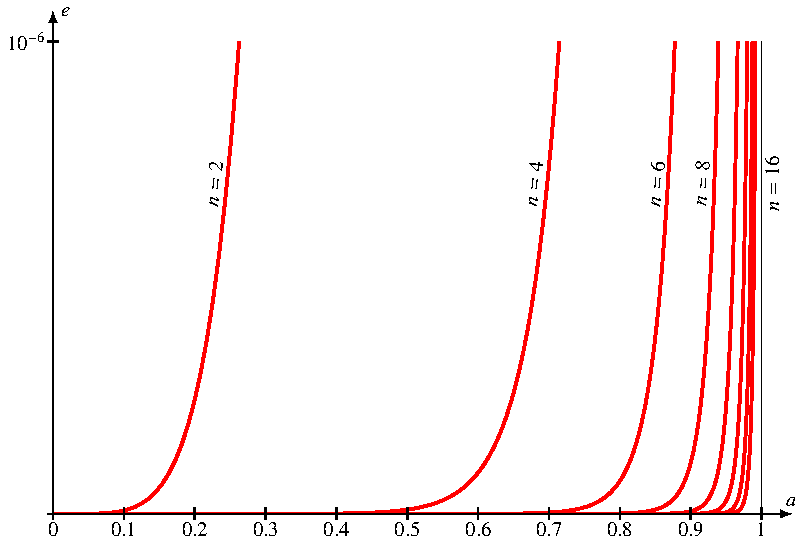
\includegraphics{chapters/060-integral/gq/gq.pdf}
\caption{Approximationsfehler des
Integrals~\eqref{buch:integral:gaussquadratur:bspintegral}
in Abhängigkeit von $a$.
Die Divergenz der Ableitung des Integranden an den Intervallenden
$\pm 1$ führt zu schlechter Konvergenz des Verfahrens, wenn $a$
nahe an $1$ ist.
\label{buch:integral:gaussquadratur:fehler}}
\end{figure}

Zur Illustration der Genauigkeit der Gauss-Quadratur berechnen wir
das Integral
\begin{equation}
\int_{-a}^a \sqrt{1-x^2}\,dx
=
\arcsin a + a \sqrt{1-a^2}
\label{buch:integral:gaussquadratur:bspintegral}
\end{equation}
mit Gauss-Quadratur einerseits und dem Trapezverfahren
andererseits.
Da Gauss-Quadratur mit sehr viel weniger Sützstellen auskommt,
berechnen wir die Trapeznäherung mit zehnmal so vielen Stützstelln.
In den Tabellen~\ref{buch:integral:gaussquadratur:table0.5}
und
\ref{buch:integral:gaussquadratur:table0.999}
sind die Resultate zusammengestellt.
Für $a =\frac12$ zeigt
Tabelle~\ref{buch:integral:gaussquadratur:table0.5}
die sehr schnelle Konvergenz der Gauss-Quadratur, schon mit
12 Stützstellen wird Maschinengenauigkeit erreicht.
Das Trapezverfahren dagegen erreicht auch mit 200 Stützstellen nur
4 korrekte Nachkommastellen.

An den Stellen $x=\pm 1$ divergiert die Ableitung des Integranden
des Integrals \eqref{buch:integral:gaussquadratur:bspintegral}.
Da grösste und kleinste Stützstelle der Gauss-Quadratur immer
deutlich vom Rand des Intervalls entfernt ist, kann das Verfahren
diese ``schwierigen'' Stellen nicht erkennen.
Tabelle~\ref{buch:integral:gaussquadratur:table0.999} zeigt, wie
die Konvergenz des Verfahrens in diesem Fall sehr viel schlechter ist.
Dies zeigt auch der Graph in
Abbildung~\ref{buch:integral:gaussquadratur:fehler}.

\subsection{Skalarprodukte mit Gewichtsfunktion}
Die Nullstellen der Legendre-Polynome ergaben ein gutes
Integrationsverfahren für Polynome auf einem beschränkten
Intervall.
Die Beispiele haben aber auch gezeigt, dass Stellen, wo die
Ableitung des Integranden divergiert, die Genauigkeit stark
beeinträchtigen können.
Ausserdem ist das Verfahren nicht anwendbar auf uneigentliche
Integrale.

\subsubsection{Umgang mit Singularitäten}
Die Lösung des Problems mit Stellen mit divergenter Ableitung
besteht darin, die Stützstellen in der Nähe dieser Stellen
zu konzentrieren.
Die Verwendung einer Gewichtsfunktion $w(x)$ kann genau dies
erreichen.
Statt das Integral einer Funktion $f(x)$ zu bestimmen, 
kann man $f(x)=g(x)w(x)$ schreiben, wobei $w(x)$ so
gewählt werden soll, dass das Verhalten der Steigung an
den Intervallenden gut wiedergibt.
Dies ist mit einer Jacobischen Gewichtsfunktion immer möglich.
Statt der Nullstellen der Legendre-Polynome sind dann die
Nullstellen der Jacobi-Polynome  und die Funktionswete von $g(x)$
an diesen Stellen zu verwenden,  die Gewichte sind
die Integrale von $l_i(x) P^{(\alpha,\beta)}(x)$.

\subsubsection{Uneigentliche Integrale}
Die Berechnung eines uneigentlichen Integrals auf dem Intervall
$(0,\infty)$ oder $(-\infty,\infty)$ ist aus mehreren Gründen nicht
direkt mit dem früher beschriebenen Gauss-Quadraturverfahren
möglich.

Die Stützstellen, die bei der Gauss-Quadratur in einem Intervall
$(a,b)$ verwendet werden, entstehen dadurch, dass man die Nullstellen
der Legendre-Polynome in $(-1,1)$ auf das Intervall $(a,b)$
skaliert.
Dies führt offensichtlich nicht zum Erfolg, wenn ein oder beide
Intervallgrenzen unendlich sind.
Dieses Problem kann dadurch gelöst werden, dass man das unendliche
Intervall $(a,\infty)$ mit
\[
x =  a + \frac{1-t}{t}
\]
auf das Intervall $[0,1]$ transformiert.

Will man beim Intervall $(0,\infty)$ bleiben, dann ist zu beachten,
dass das Integral eines Polynomes immer divergent ist, es ist also
auf jeden Fall nötig, den Integranden durch Funktionen zu approximieren,
die genügend schnell gegen $0$ gehen.
Polynome beliebigen Grades können verwendet werden, wenn sie mit
einer Funktion multipliziert werden, die schneller als jedes Polynom
gegen $0$ geht, so dass das Integral immer noch konvergiert.
Die Funktionen $e^{-x}$ für das Intervall $(0,\infty)$ oder
$e^{-x^2}$ für das Intervall $(-\infty,\infty)$ kommen dafür in Frage.

Um das Integral von $f(x)$ im Intervall $(0,\infty)$ zu berechnen,
schreibt man daher zunächst
\[
\int_0^\infty f(x)\,dx
=
\int_0^\infty g(x)e^{-x}\,dx
=
\int_0^\infty g(x) w(x)\,dx
\quad\text{mit}\quad
w(x)=e^{-x}
\text{ und }
g(x)=f(x)e^x.
\]
Dann approximiert $g(x)$ man durch ein Interpolationspolynom,
so wie man das bei der Gauss-Quadratur gemacht hat.
Als Stützstellen müssen dazu die Nullstellen der Laguerre-Polynome
verwendet werden.
Als Gewichte $w_i$ sind die Integrale der $l_i(x)e^{-x}$
zu verwenden.







